\documentclass[12pt]{article}


\author{Daniel Eberharter\\ Claudio Canella}
\title{Ridge regression}

\usepackage{amsmath}
\usepackage{graphicx}
\usepackage{float}
\floatplacement{figure}{H}
\usepackage[margin=1in]{geometry}


\begin{document}
\maketitle


\section{Algorithmic Choices}
Our method does not substantially differ from the one discussed in class. We chose two non-linear functions, one is $f(x) = x^2 + 2x + 2$ and the other one is $g(x) = 6x^2 + 2x + 2$. We then determine our data sets by calculating $r^t(x) = f(x^t) + \epsilon$ (and $r^t(x) = g(x^t) + \epsilon$ respectively for $g(x)$), where $\epsilon$ is drawn from a standard uniform distribution with a random error selected between 0 and 15 weighted by the variance(for full information on calculation please see the octave script). The x-values are linear distributed between $x_{min}$ and $x_{max}$ \\
We calculate our design matrix and use the formula that has been introduced in the lecture and further determine the coefficients $w_i$ for the regression function  for each given value of $\lambda$ (to avoid biasing towards $w_0$ the y-values are centered). \\
By using M-fold cross-validation we find the best $\lambda$ out of the chosen values.
\pagebreak

\section{Numbers and Illustrations}
	\begin{itemize} \label{plotted}
		\item $x_{min} = 0, x_{max} = 9, x_n = 20$
		\item $M = 3$
		\item probability of error: 15\% (used for $\epsilon$)
		\item $\lambda$ values are logarithmic equally distributed between $\lambda_{min} = 1$ and $\lambda_{max} = 10^6$, $\lambda_n = 19$
		\item The $\lambda_i$ to be plotted are selected as follows (where b is the index of the best $\lambda$)
			\[ \lambda_{b} \]
			\[ \lambda_{1+(b - \frac{\lambda_n}{2}) \% \lambda_n} \]
			\[ \lambda_{\lambda_n -( 1+(b - \frac{\lambda_n}{2}) \% \lambda_n}\]
	\end{itemize}

	\begin{figure}
		\centering
		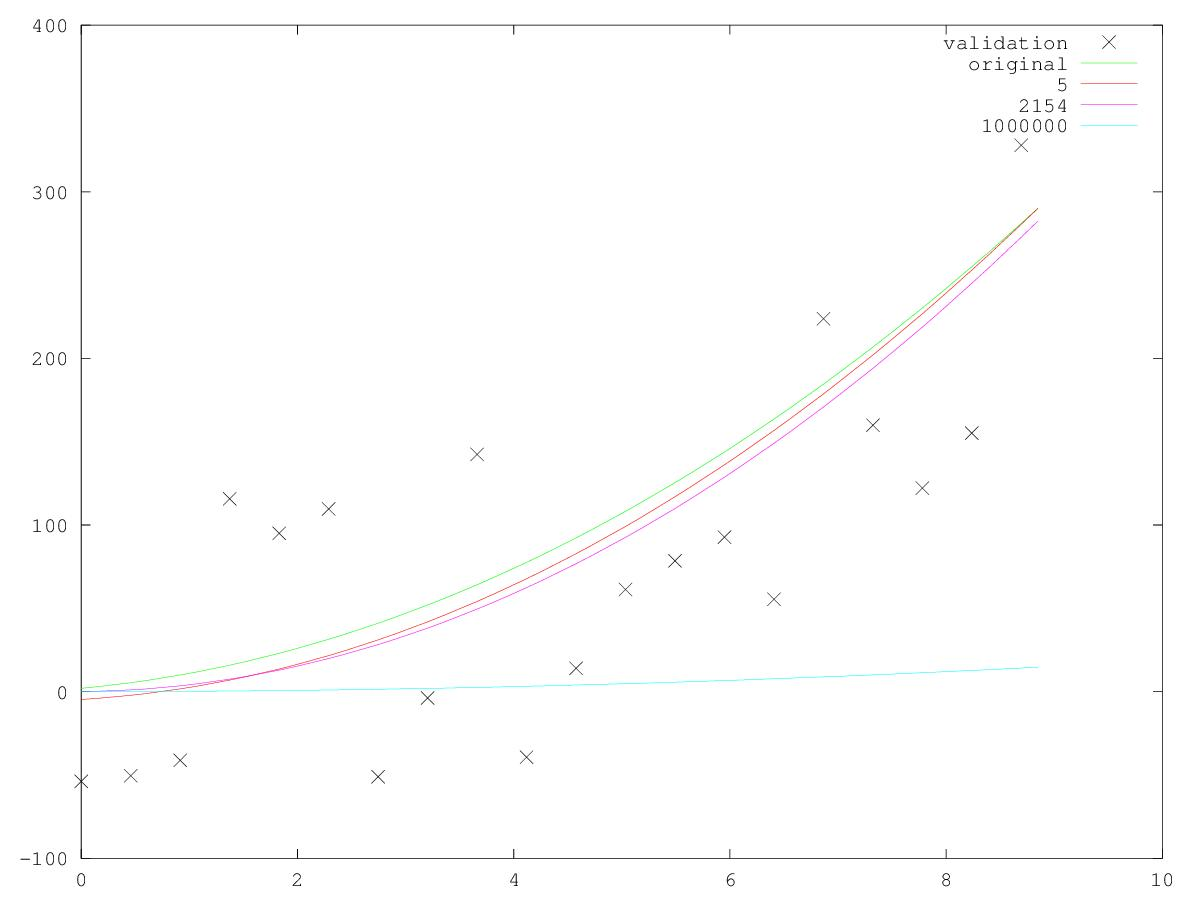
\includegraphics[scale=0.5]{plot}
		\caption{g(x) with 3 approximations (with the noted $\lambda$ value) and the respective validation set}
		\label{fig:small_g_plot}
	\end{figure}

	\begin{figure}
		\centering
		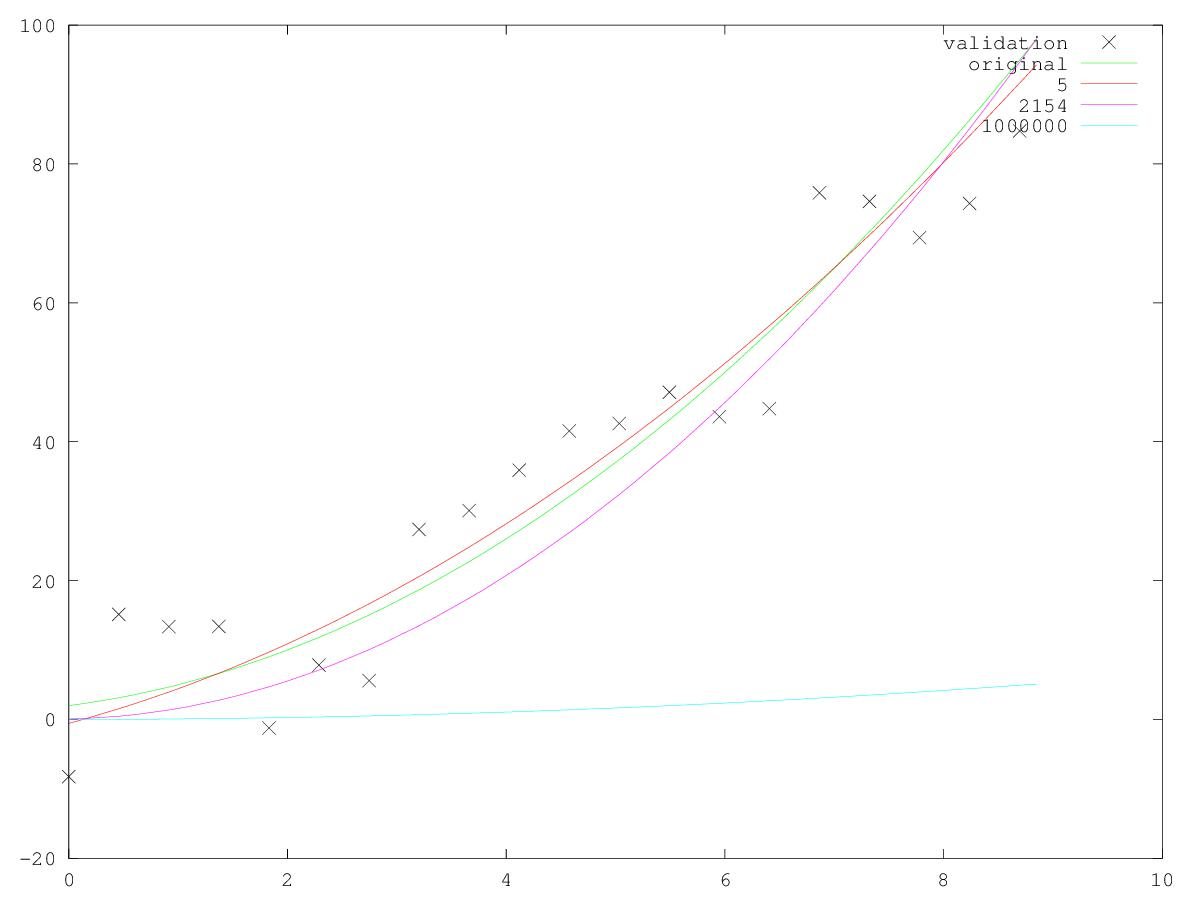
\includegraphics[scale=0.5]{small_f_plot}
		\caption{f(x) with 3 approximations (with the noted $\lambda$ value) and the respective validation set}
		\label{fig:small_f_plot}
	\end{figure}
 
As it is part of the task, we created a plot with $\lambda$ on the abscissa and the error on the ordinate as it can be seen in figures \ref{log_1} and \ref{log_2}. 
In figures \ref{clog_1} and \ref{clog_2} we can see all the calculated errors for both functions with the best one being indicated.

	\begin{figure}
		\centering
		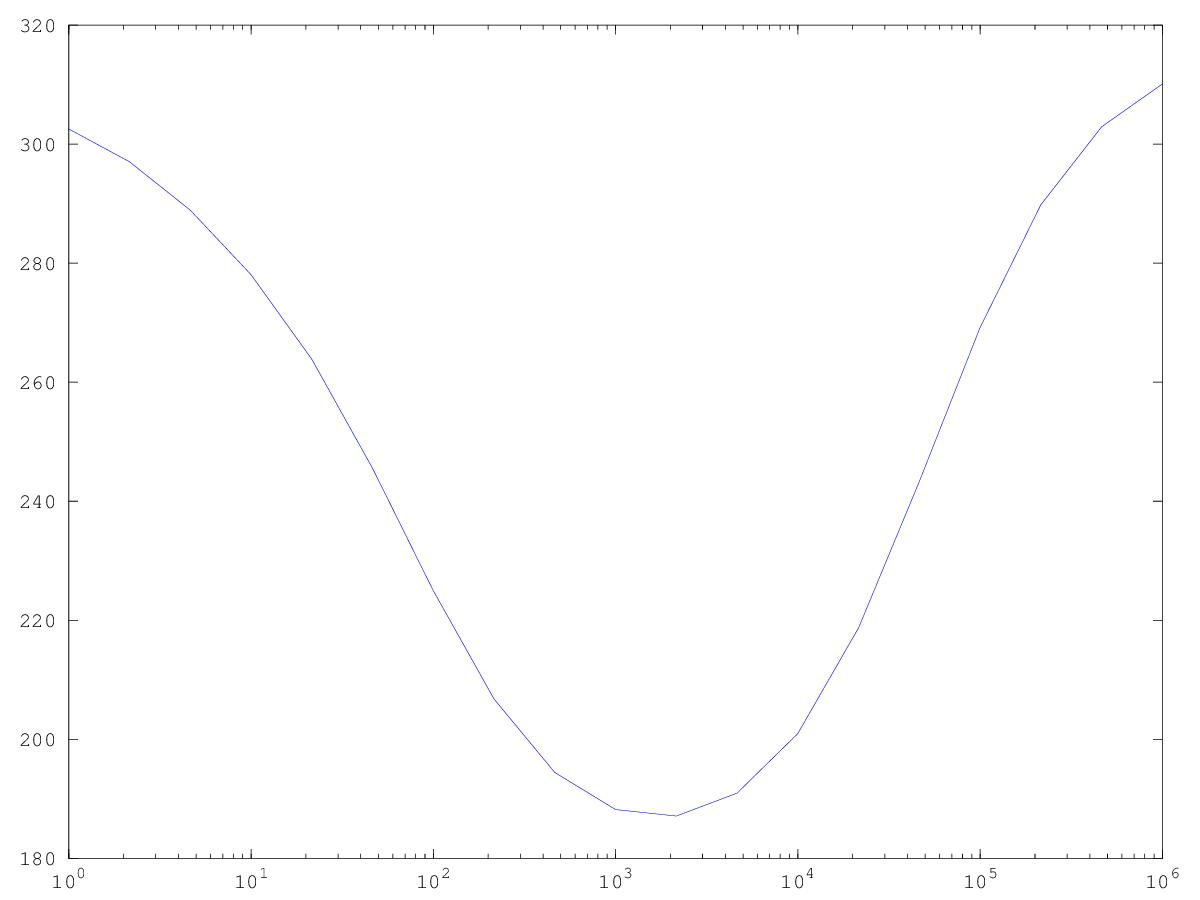
\includegraphics[scale=0.5]{log}
		\caption{ $\lambda$ and the error plotted on a logarithmic abscissa for $f(x) = 3x^2 + 6x + 2$}
		\label{log_1}
	\end{figure}

	\begin{figure}
		\centering
		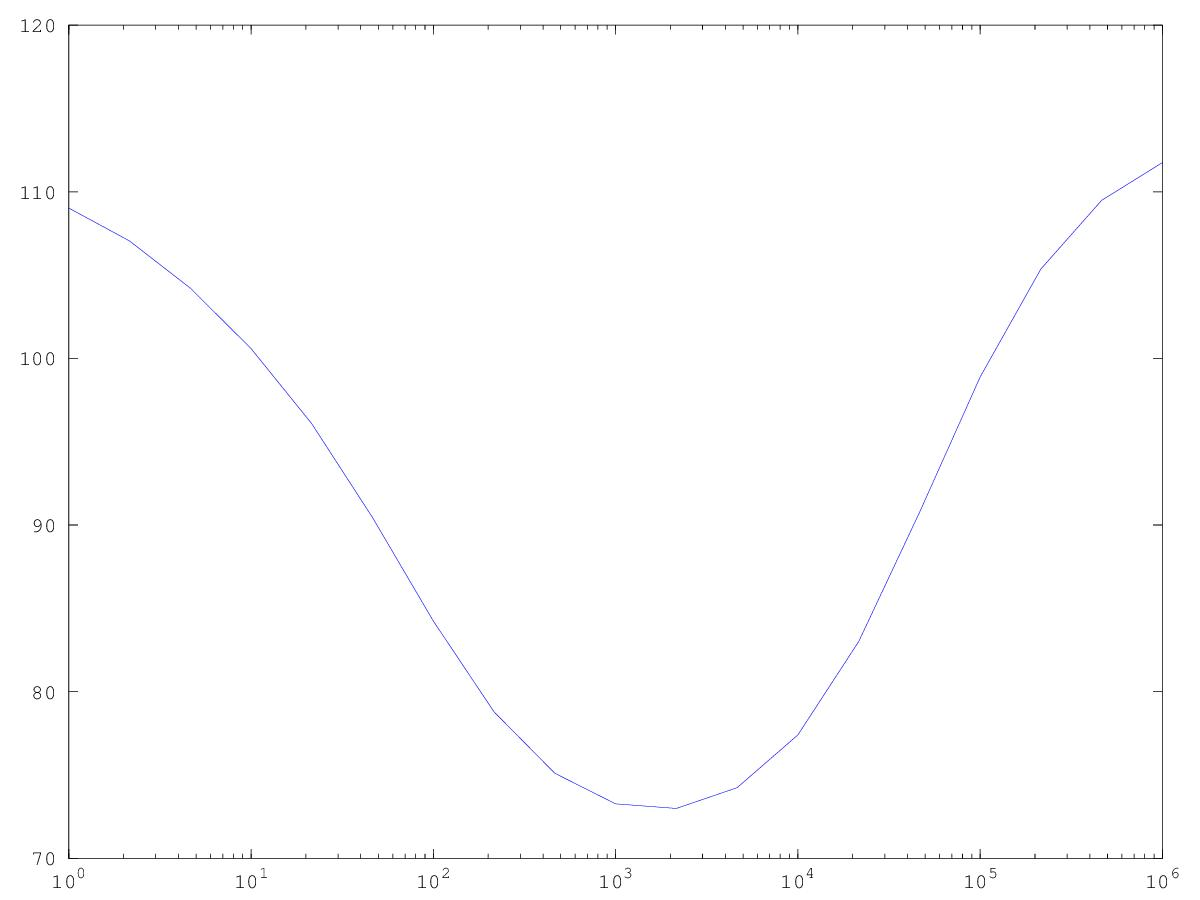
\includegraphics[scale=0.5]{log_small_f}
		\caption{ $\lambda$ and the error plotted on a logarithmic abscissa for $f(x) = x^2 + 2x + 2$}
		\label{log_2}
	\end{figure}
	
	\begin{figure}
		\centering
		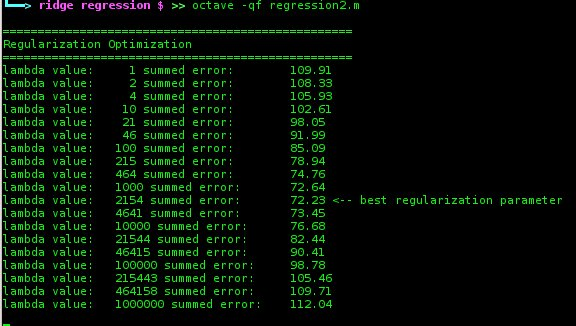
\includegraphics[scale=0.7]{console_output_small_f}
		\caption{ $\lambda$ and the error for $f(x) = x^2 + 2x + 2$}
		\label{clog_1}
	\end{figure}

	\begin{figure}
		\centering
		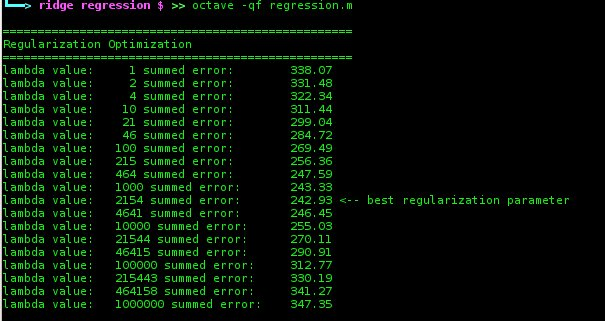
\includegraphics[scale=0.7]{console_output_big_f}
		\caption{ $\lambda$ and the error for $g(x) = 3x^2 + 6x + 2$}
		\label{clog_2}
	\end{figure}

\section{Conclusion}
We tested our implementation with different functions without increasing the order of our polynomial as we would have to change the whole implementation of the program. Instead we increased and decreased the weighting factor of each order and our $\lambda$ values. While doing this we noticed that for the function with the higher slope($g(x) = 3x^2 + 6x + 2$) our approximation with the different $\lambda$ values is almost identical for small x-values, but with increasing x the regression function will diverge, as seen in figure \ref{fig:plot}. \\
When we use the function with the lower slope($f(x) = x^2 + 2x + 2$) it is the other way around, meaning that the approximation with the different $\lambda$ values diverge with small x values and converge with bigger x, as seen in figure \ref{fig:small_f_plot}. \\
As seen in figures \ref{log_1} and \ref{log_2} the selection of the regularization parameter $\lambda$ can have a significant influx on the error of the regression function. Nevertheless this parameter should be chosen carefully because a too big value for $\lambda$ can increase the error as well (with the limit being a linear regression function with no relation to the original function).

\end{document}
